% Chapter 1

\chapter{Introducción general} % Main chapter title

\label{Chapter1} % For referencing the chapter elsewhere, use \ref{Chapter1} 
\label{IntroGeneral}

%----------------------------------------------------------------------------------------

% Define some commands to keep the formatting separated from the content 
\newcommand{\keyword}[1]{\textbf{#1}}
\newcommand{\tabhead}[1]{\textbf{#1}}
\newcommand{\code}[1]{\texttt{#1}}
\newcommand{\file}[1]{\texttt{\bfseries#1}}
\newcommand{\option}[1]{\texttt{\itshape#1}}
\newcommand{\grados}{$^{\circ}$}

%----------------------------------------------------------------------------------------

%\section{Introducción}

Este capítulo presenta una introducción a los conceptos básicos de la temática del trabajo y explica las principales causas que motivaron el desarrollo del proyecto, junto con los objetivos que se buscaron alcanzar.

%----------------------------------------------------------------------------------------
\section{Planteo básico}

Existen en la actualidad diferentes soluciones en lo que respecta a la prevención o seguridad ciudadana \citep{PNUD:1}. Estos sistemas centralizan información en tiempo real de cámaras de seguridad, móviles de las fuerzas de seguridad, entre otros. Además, suelen incorporar alguna funcionalidad para que un ciudadano, ante una situación de emergencia, pueda dar aviso a las autoridades. El mecanismo para notificar puede ser una aplicación móvil, un dispositivo geolocalizador u otra alternativa pero el objetivo es el mismo. En la figura 1.1 se pueden observar los componentes de alto nivel del sistema web y del dispositivo geolocalizador.

\begin{figure}[htbp]
	\centering
	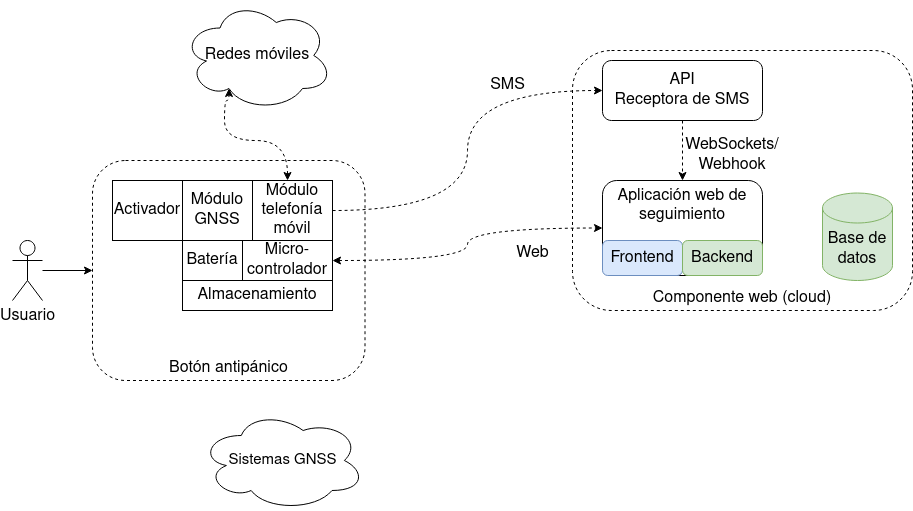
\includegraphics[width=.9\textwidth]{./Figures/diagBloques.png}
	\caption{Diagrama en bloques del dispositivo y el sistema web}
	\label{fig:texmaker}
\end{figure}

\subsection{Botones antipánico}

Un botón antipánico hace referencia a un dispositivo pequeño y portátil, alimentado por batería, que permite a una persona, ante una situación de emergencia, presionar un pulsador con el objetivo de generar una alerta y que esta sea recepcionada en un sistema de monitoreo.

Estos dispositivos generalmente son brindados por las autoridades, aunque también también pueden ser provistos por empresas de seguridad privadas. Sus beneficiarios suelen ser:
\begin{itemize}
\item Personas en situación de violencia de género.	
\item Personas en situación de violencia intrafamiliar.
\item Establecimientos donde pueden ocurrir situaciones de violencia y es necesario dar rápidamente aviso a las autoridades.
\item Agente o sereno cuyo recorrido debe ser registrado.
\end{itemize}
Entre otros.

Entre sus funcionalidades, suelen poseer:
\begin{itemize}
\item Conectividad a la red de telefonía móvil (\textit{Global System for Mobile communications} o GSM).
\item Acceso a datos móviles (\textit{General Packet Radio Service} o GPRS).
\item Conectividad a sistemas de geoposicionamiento satelital (\textit{Global Navigation Satellite System} o GNSS).
\item Botón de disparo de alerta.
\item Reporte periódico de ubicación por mensaje de texto (SMS) o vía web.
\end{itemize}

Un detalle interesante respecto a estos dispositivos es que generalmente se comercializan en dos formatos:

\begin{itemize}
\item Dispositivo personal: dispositivo embebido que puede ser llevado como colgante, en la muñeca o en el bolsillo. Tiene una autonomía limitada.
\item Dispositivo para móviles: también conocido como AVL o \textit{Automatic Vehicle Location}; además de contar con antenas externas para mayor precisión, cuenta con cables para conexión a la batería de los vehículos, permitiendo tener una mayor autonomía.
\end{itemize}


En relación a este trabajo, se planteó el desarrollo del prototipo de un botón geolocalizador y una plataforma web a modo de prueba de concepto, para la recepción de alertas.

%----------------------------------------------------------------------------------------

\section{Motivación}

El autor del trabajo posee experiencia en este tipo de soluciones, principalmente en la adquisición, configuración, implementación y soporte de botones antipánico disponibles en el mercado. Se detectó y se llegó a la conclusión, respecto a los dispositivos, de que estos presentan los siguientes inconvenientes:

\begin{itemize}
\item Especificaciones de hardware obsoletas.
\item Documentación escasa, desactualizada o incluso incorrecta en algunos casos.
\item Poca fiabilidad de dispositivo (dificultad para configurarlos, mala señal en ambientes \textit{indoor}, desconfianza al momento de utilizarlo).
\item Inconsistencias entre dispositivos idénticos.
\item Poca duración de batería (desde aproximadamente 24 horas hasta 3 o 4 días como máximo, cuando lo deseable para el beneficiario final del botón es de al menos 5 o 6 días).
\item Precio exageradamente elevado y muchas dificultades para adquirirlos mediante proveedores, más en períodos de alta inflación.
\item Nulas características de seguridad.
\end{itemize}

Se investigaron y revisaron diferentes alternativas en el mercado, así como también se trabajó con dispositivos utilizados por sistemas de la competencia, llegando a conclusiones similares: no se encuentran dispositivos aceptables cuyo costo sea accesible.

Todas estas cuestiones nombradas anteriormente son las que motivaron la formulación del proyecto, siendo necesario disponer de un dispositivo embebido funcional y un sistema web que permita recepcionar la información del botón.

Otras motivaciones menores del trabajo, pero igualmente muy relacionadas a la especialización, fueron:
\begin{itemize}
\item Profundizar en el uso de frameworks para \textit{Single Web Applications} o SPAs.
\item Poder aplicar los conocimientos trabajados en relación a tecnologías \textit{cloud} y desarrollo de APIs web.
\end{itemize}

%----------------------------------------------------------------------------------------

\section{Objetivos y alcance}

En relación a los objetivos de alto nivel del trabajo, estos fueron:
\begin{itemize}
\item Investigación y determinación de un conjunto de módulos de hardware que sean adecuados para la construcción del prototipo.
\item Diseño y construcción un prototipo de botón antipánico que permita validar las decisiones tecnológicas.
\item Tener fiabilidad superior sobre ciertas características, en comparación con algunos de los dispositivos disponibles en el mercado.
\item Desarrollo de un sistema web a modo de prueba de concepto para el uso del dispositivo.
\end{itemize}

Respecto a los objetivos por componente, estos se presentan en la tabla 1.1.

\begin{table}[h]
	\centering
	\caption[Resumen de objetivos]{Resumen de objetivos del trabajo}
	\begin{tabular}{l c c}    
		\toprule
		\textbf{Componente} 	 & \textbf{Objetivo} 	  \\
		\midrule
		Prototipo & Duración de la batería 				\\		
		Prototipo & Calidad de señal de GSM en ambientes cerrados y abiertos			\\
		Prototipo & Calidad de señal de GNSS en ambientes cerrados y abiertos			\\
		Prototipo & Tiempo de actualización de la ubicación (\textit{time-to-first-fix}) \\
		Prototipo & Envío de alertas mediante pulsador		\\
		Sistema web & Recepción de SMS de alertas			\\
		Sistema web & Alta de dispositivos			\\
		Sistema web & Visualización de alertas en tiempo real			\\
		Sistema web & Despliegue en un entorno \textit{cloud}			\\
		\bottomrule
		\hline
	\end{tabular}
	\label{tab:peces}
\end{table}

No se incluyeron, dentro del alcance del trabajo, las siguientes características:

\begin{itemize}
\item Aplicación web productiva para gestionar las activaciones del botón antipánico. Por productiva se refiere a que pueda ser ofrecida al mercado o utilizable por usuarios encargados del monitoreo.
\item Desarrollo de un dispositivo listo para reemplazar dispositivos existentes, es decir que no sea un prototipo.
\item Desarrollo de un contenedor físico para el dispositivo.
\end{itemize}

Además, durante el desarrollo del trabajo, se fueron detectando diferentes cuestiones técnicas a resolver, que modificaron algunos objetivos planteados inicialmente.

%----------------------------------------------------------------------------------------

\section{Soluciones comerciales similares}

Se presentan a continuación algunos modelos conocidos y utilizados en el mercado local. Estos dos modelos sufren los inconvenientes nombrados en las secciones anteriores: el motivo de fondo es que existen muchos clones de estos modelos, resultando muy difícil determinar si se está trabajando con un dispositivo original o un clon con posibles problemas \citep{CLONES:1}.
\subsection{LK109}

LK109 es el nombre de un dispositivo geolocalizador que trabaja con redes GSM y GPRS, y usa \textit{Global Positioning System} (GPS) como sistema de GNSS. Existe también una versión que trabaja con redes 3G, cuyo costo es superior. En la figura 1.2 se puede observar el dispositivo en cuestión.

\begin{figure}[H]
	\centering
	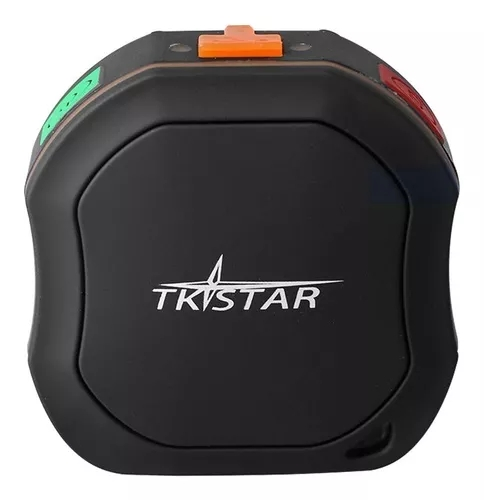
\includegraphics[width=.6\textwidth]{./Figures/lk109.jpg}
	\caption{Imagen del botón LK109}
	\label{fig:texmaker}
\end{figure}
Entre sus características más interesantes se encuentran \citep{LK109MANUAL:1}:
\begin{itemize}
\item Indicadores de estado: batería, señal de GPS y señal de GSM.
\item Posibilidad de reportar la ubicación mediante TCP o SMS.
\item Reporte de ubicación en tiempo real, con una perioricidad configurable.
\item Posibilidad de monitorear de forma remota el entorno del dispositivo mediante un micrófono.
\item Autonomía de 240 horas o 10 días.
\end{itemize}



\subsection{TK102B}

TK102B es el nombre de otro dispositivo geolocalizador que trabaja con redes GSM y GPRS, y usa \textit{Global Positioning System} (GPS) como sistema de GNSS. En la figura 1.3 puede observarse el diseño de este modelo de dispositivo.

\begin{figure}[H]
	\centering
	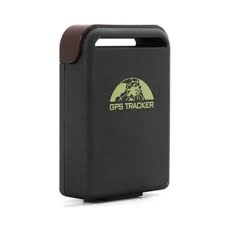
\includegraphics[width=.6\textwidth]{./Figures/tk102b.jpg}
	\caption{Imagen del botón TK102B}
	\label{fig:texmaker}
\end{figure}

Entre sus características más relevantes se encuentran \citep{TK102BMANUAL:1}:
\begin{itemize}
\item Indicadores de estado: batería, señal de GPS y señal de GSM.
\item Posibilidad de reportar la ubicación mediante TCP o SMS, incluyendo la dirección aproximada, mediante geodecodificación inversa.
\item Reporte de ubicación en tiempo real, con una periodicidad configurable.
\item Posibilidad de monitorear de forma remota el entorno del dispositivo mediante un micrófono.
\item Autonomía de 80 horas o 3 días aproximadamente.
\end{itemize}


Se presentan a continuación las principales características de estos dos modelos, contrastadas:

\begin{table}[H]
	\centering
	\caption[Tabla comparativa]{Tabla comparativa de los dos modelos}
	\begin{tabular}{l c c}    
		\toprule
		\textbf{Característica} 	 & \textbf{LK109} & \textbf{TK102B}	  \\
		\midrule
		Conectividad & GSM, GPRS, SMS & 	GSM, GPRS, SMS			\\		
		Reporte periódico & Sí & Sí			\\
		Autonomía (horas) & 240 & 80		\\
		Indicadores de estado & Sí & Sí \\
		Escucha remota & Sí & Sí \\
		Protocolo de comunicación & h02 & gps103 \\
		\bottomrule
		\hline
	\end{tabular}
	\label{tab:peces}
\end{table}

Respecto al ítem de autonomía, no se ha podido comprobar en la práctica que la duración sea la indicada (siempre es mucho menor, entre 12 y 24 horas), a excepción del uso mediante \textit{sleep} o ahorro de batería, que no tiene utilidad para las aplicaciones de seguimiento de una persona. Esto es debido a que, en el modo de ahorro de batería, la ubicación se actualiza posterior al envío de una alerta y no antes, resultando inútil la ubicación reportada.

En relación al ítem de escucha remota, es decir la posibilidad de escuchar lo que ocurre alrededor del dispositivo, no se ha podido verificar para varios dispositivos; de todas maneras no resulta una funcionalidad útil en la mayoría de los casos de uso. Las características que se deben cumplir y validar obligatoriamente son:
\begin{itemize}
	\item Precisión al momento de obtener la ubicación.
	\item Autonomía considerable de la batería.
	\item Rapidez para obtener señal de GSM y GNSS.
\end{itemize}